\chapter{Systems of sparse polynomial equations}

\scribe{Anna Somoza}
 
\textbf{Goal:} Our aim is to construct systems of sparse polynomial equations with non-trivial lower-bound on the number of real solutions.

\textbf{Motivation:} We think abount this problem inspired by Kouchironko bound: Given the polynomial system
$$\begin{cases}
F_1(x_1,\dots,x_n) = 0\\
\vdots\\
F_n(x_1,\dots,x_n) = 0\\
\end{cases}$$

such that they share the same Newton polynomial $N(F_i)$, then we get that the number of complex solutions for the system is $\operatorname{vol} N(F_i)$.


\textbf{Tools:} We will introduce:
\begin{enumerate}
\item A generalization of Veronese embedding,
\item replace system of polynomial equations in
$$(\CC^*)^n = \CC^n \backslash \{\bigcup_i\{x_i = 0\}\}$$
by a system of linear equations in $\mathbb{P}^{\Delta \cap \ZZ^n} = \mathbb{P}^\Delta$:
\begin{align*}
\varphi_\Delta : (\CC^*)^n  &\to \mathbb{P}^\Delta\\
(t_1,\dots,t_n) &\mapsto [t^m : m\in \Delta \cap \ZZ^n]
\end{align*}
\end{enumerate}

\begin{example}
For $n = 1$
\begin{align*}
\varphi_\Delta : \CC^*  &\to \mathbb{P}^\Delta\\
t &\mapsto [1:t:t^2:t^3]
\end{align*}
\end{example}

- Degree of a map between orientable mainfolds:

$X_\Delta = \operatorname{cl}(\Im \varphi_\Delta)$ in a Zariski topology

toric ($(\CC^*)^n$ acts on $X_\Delta$) variety associated to $\Delta$.



\section{Wronski polynomials}

We require a foldable (i.e. rainbow colored), full and regular triangulation of $L$.

\begin{definition}
A triangulation $T$ is said to be foldable if there exists a graph homomorphism such that
$$\operatorname{sk}^1(T) = \operatorname{sk}^1(\conv\{0,e_1,\dots,e_n\}).$$

It is equivalent to say that it is foldable if and only if its dual graph is bipartite.
\end{definition}

\begin{figure}
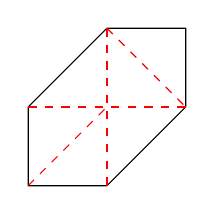
\begin{tikzpicture}
\draw (0,0) -- (1,0) -- (2,1) -- (2,2) -- (1,2) -- (0,1) -- cycle;
\draw[red, dashed] (0,0) -- (1,1);
\draw[red, dashed] (0,1) -- (1,1);
\draw[red, dashed] (1,0) -- (1,1);
\draw[red, dashed] (1,2) -- (1,1);
\draw[red, dashed] (2,1) -- (1,1);
\draw[red, dashed] (1,2) -- (2,1);
\end{tikzpicture}
\caption{A non-foldable triangulation}
\end{figure}

\begin{figure}
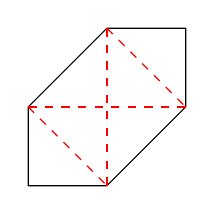
\begin{tikzpicture}
\draw (0,0) -- (1,0) -- (2,1) -- (2,2) -- (1,2) -- (0,1) -- cycle;
\draw[red, dashed] (0,1) -- (1,0);
\draw[red, dashed] (0,1) -- (1,1);
\draw[red, dashed] (1,0) -- (1,1);
\draw[red, dashed] (1,2) -- (1,1);
\draw[red, dashed] (2,1) -- (1,1);
\draw[red, dashed] (1,2) -- (2,1);
\end{tikzpicture}
\caption{A non-foldable triangulation}
\end{figure}


\begin{definition}
We say that a triangulation is full if and only if
$$\operatorname{sk}^0 T = \Delta \cap \ZZ.$$
\end{definition}

\begin{definition}
We say that a triangulation is regular if and only if it is induced by a convex height function on $\Delta \cap \ZZ^n$
\end{definition}
% Local Variables: 
% mode: pdflatex
% TeX-master: "dag-upc"
% End: 
